
En este último experimento del trabajo practico, se pretende medir el factor de potencia del circuito, con un medidor digital de potencia que se puede ver en la figura \ref{fig:mediPot}. Este dispositivo es modelo TS 836, de la marca Stand-By. 

Este medidor, se utiliza conectándolo al toma corriente y conectando el circuito a medir, en su propia salida de toma corriente. En otras palabras, se conecta como un adaptador o protector de sobre-tensión.

\begin{figure}[H]
    \begin{subfigure}{0.6\textwidth}
        \centering
        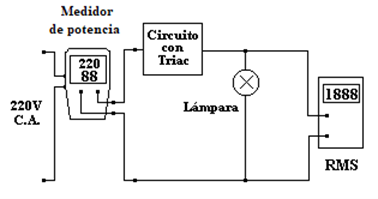
\includegraphics[width=1\textwidth]{Imagenes/exp5med.png}
     \caption{Circuito experimento 5}
     \label{fig:exp5med}
    \end{subfigure}
    \hspace*{\fill}
    \begin{subfigure}{0.39\textwidth}
        \centering
        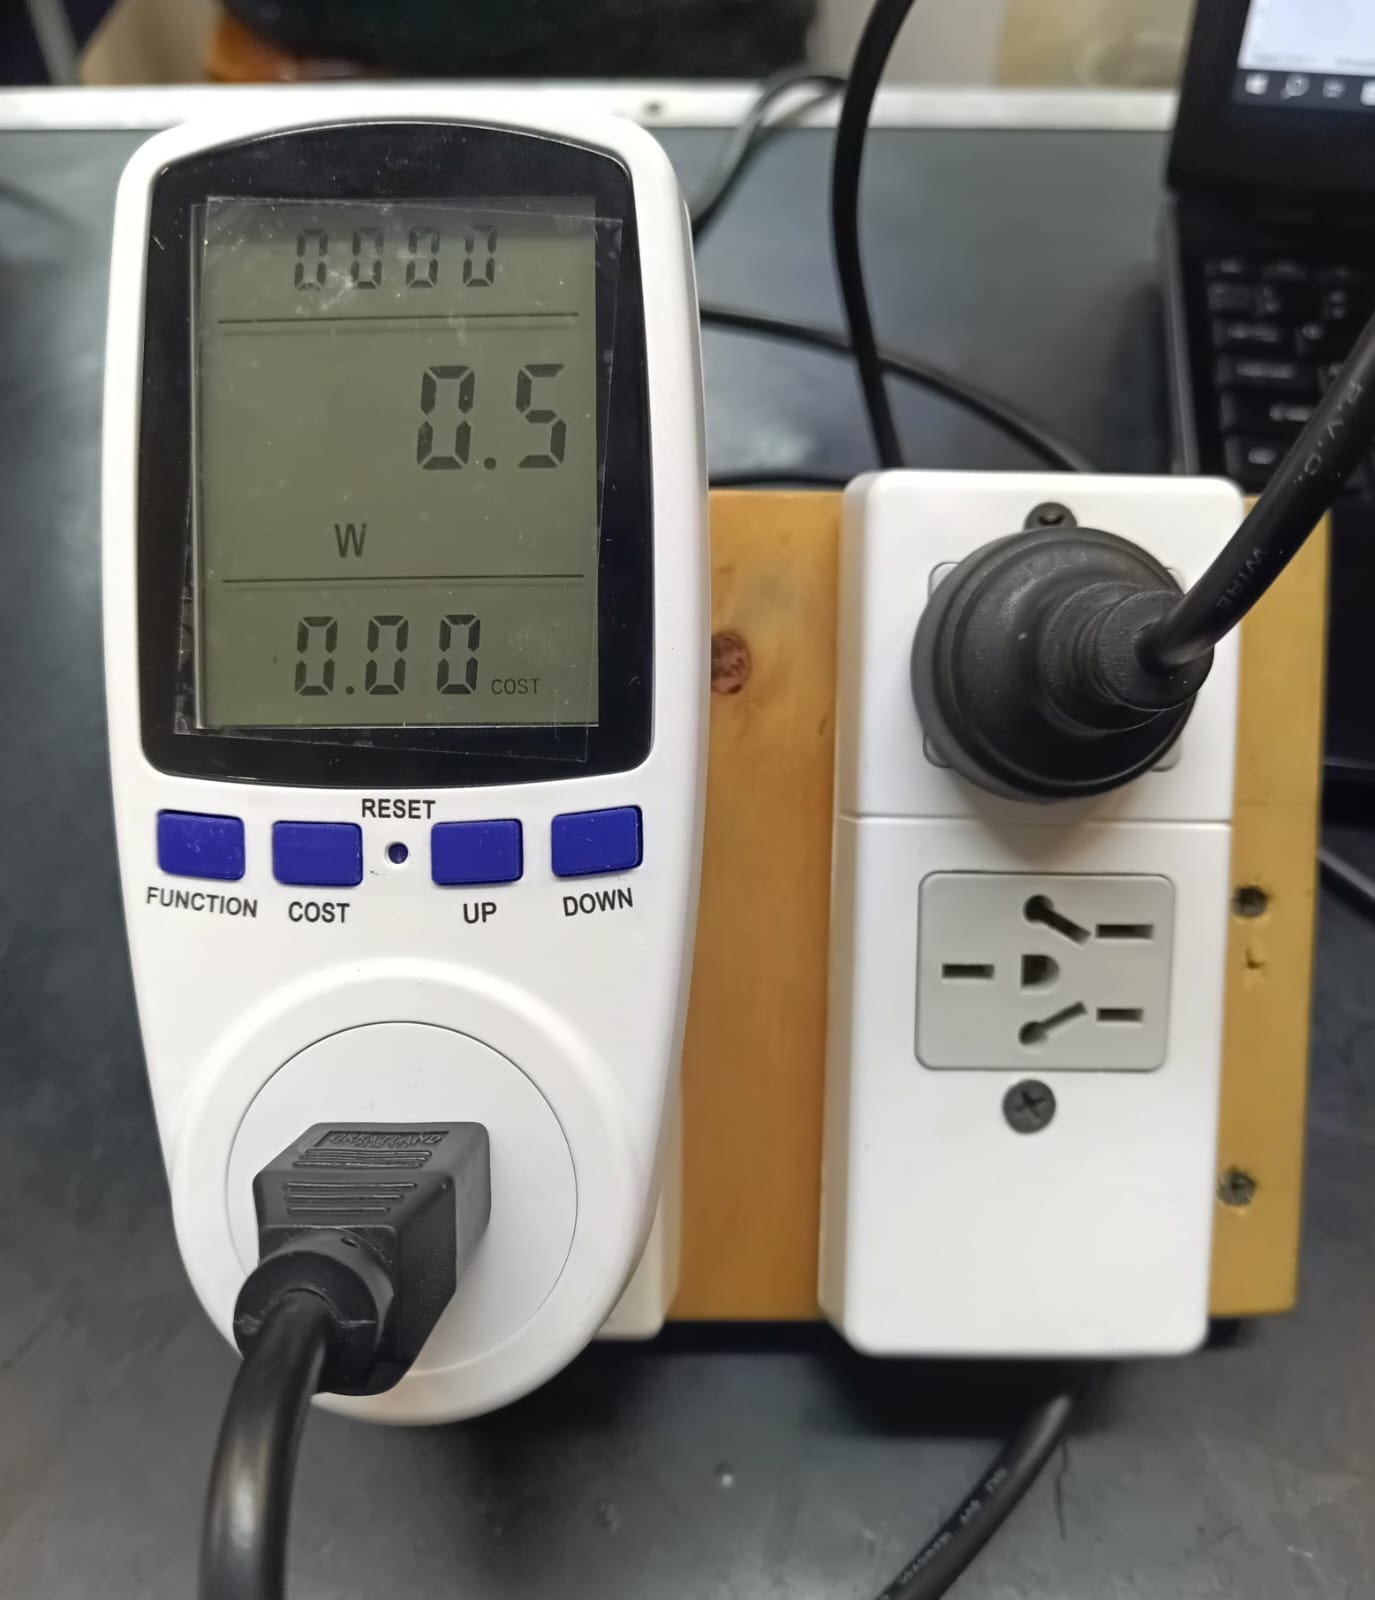
\includegraphics[width=0.7\linewidth]{Imagenes/mediPot.jpeg}
        \caption{Medidor digital de Potencia}
        \label{fig:mediPot}
    \end{subfigure}
    \caption{Circuito y medidor utilizados}
\end{figure}

Como se ve en la figura \ref{fig:exp5med}, se debe conectar el circuito de control de ángulo de conducción al medidor de potencia como se describió en el párrafo anterior.

Una vez conectado, se modificó el potenciómetro de tal manera, para que la lampara esté alimentada con una tensión eficaz de $V_i=110V$ aproximadamente. El objetivo es obtener el factor de potencia del circuito en estas condiciones y determinar si la carga es capacitiva o inductiva.

\unsubsubsection{Mediciones}

Con todo conectado, se procedió a medir la potencia activa disipada por el circuito y su factor de potencia. Los datos fueron los siguientes:

\begin{equation*}
    V_L = 230.7 ~V \hspace{10mm} I = 0.138 ~A \hspace{10mm}
    P = 14.1 ~W \hspace{10mm} \cos (\phi) = 0.44
\end{equation*}

Se puede ver que el dispositivo marca que hay un desfase entre la tensión de entrada y la corriente, y la consigna de este experimento pedía que en base a este dato, se averiguara si la carga era de carácter capacitivo o inductivo.

Sin embargo, el circuito conectado, constaba de una lampara incandescente (resistencia) con un circuito de disparo por TRIAC. Y en el experimento anterior, se verificó en la figura \ref{fig:fot_exp4}, que las señales de entrada y de salida (con ángulo de conducción) están en fase. Por lo que se puede comprobar que la medición de factor de potencia (o coseno de fi), es errónea, ya que fi ($\phi$) es en realidad igual a 0, ergo el factor de potencia es igual a 1.

Este error en la detección del factor de potencia puede haberse producido debido a que el medidor de potencia está preparado para analizar desfasamiento entre dos señales sinusoidales, en cambio en este caso, una de ellas es una senoidal recortada. 

Según nos explicó uno de los docentes, comúnmente para medir el desfasamiento entre señales, el circuito interno busca los cruces por cero de la señal. Y como la señal recortada tiene los cruces por cero de manera irregular (o al menos para el medidor), este se confunde y al no poder procesar esta diferencia de forma entre las señales, muestra lo que el cree que es el factor de potencia.

%(figura \ref{fig:exp5m}):

